

\chapter{薛宝钗小恙梨香院\hspace{.5em}贾宝玉大醉绛芸轩}
{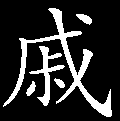
\includegraphics[width=3mm]{../Images/00005}\kaishu 幻情浓处故多嗔,岂独颦儿爱妒人。莫把心思劳展转,百年事业总非真。}

题曰:

古鼎新烹凤髓香,那堪翠斝贮琼浆。

莫言绮縠无风韵,试看金娃对玉郎。

话说凤姐和宝玉回家,见过众人。宝玉先便回明贾母,秦钟要上家塾之事,自己也有了个伴读的朋友,正好发奋,{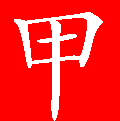
\includegraphics[width=3mm]{../Images/00002}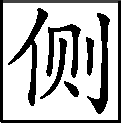
\includegraphics[width=3mm]{../Images/00011}\footnotesize \kaishu 未必。}又着实的称赞秦钟的人品行事,最使人怜爱。{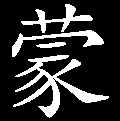
\includegraphics[width=3mm]{../Images/00006}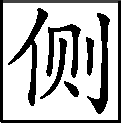
\includegraphics[width=3mm]{../Images/00011}\footnotesize \kaishu “怜爱”二字写出宝玉真神,若是别个断不肯透露。}凤姐又在一旁帮着说“过日他还来拜老祖宗”等语,{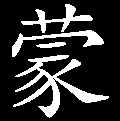
\includegraphics[width=3mm]{../Images/00006}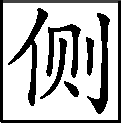
\includegraphics[width=3mm]{../Images/00011}\footnotesize \kaishu 凤姐帮话是为秦氏,用意屈尽人情。}说的贾母喜悦起来。{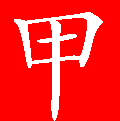
\includegraphics[width=3mm]{../Images/00002}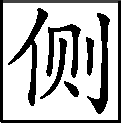
\includegraphics[width=3mm]{../Images/00011}\footnotesize \kaishu 止此便十成了,不必繁文再表,故妙。偷渡金针法。}凤姐又趁势请贾母后日过去看戏。贾母虽年高,却极有兴头。{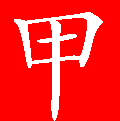
\includegraphics[width=3mm]{../Images/00002}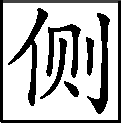
\includegraphics[width=3mm]{../Images/00011}\footnotesize \kaishu 为贾母写传。}至后日,又有尤氏来请,遂携了王夫人、林黛玉、宝玉等过去看戏。至晌午,贾母便回来歇息了。{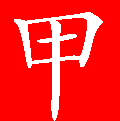
\includegraphics[width=3mm]{../Images/00002}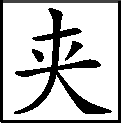
\includegraphics[width=3mm]{../Images/00012}\footnotesize \kaishu 叙事有法,若只管写看戏,便是一无见世面之暴发贫婆矣。写“随便”二字,兴高则往,兴败则回,方是世代封君正传。且“高兴”二字,又可生出多少文章来。}王夫人本是好清净的,{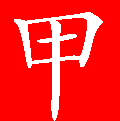
\includegraphics[width=3mm]{../Images/00002}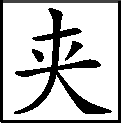
\includegraphics[width=3mm]{../Images/00012}\footnotesize \kaishu 偏与邢夫人相犯,然却是各有各传。}见贾母回来,也就回来了。然后凤姐坐了首席,尽欢至晚无话。{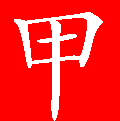
\includegraphics[width=3mm]{../Images/00002}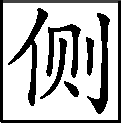
\includegraphics[width=3mm]{../Images/00011}\footnotesize \kaishu 细甚,交代毕。}

却说宝玉因送贾母回来,待贾母歇了中觉,意欲还去看戏取乐,又恐扰的秦氏等人不便,{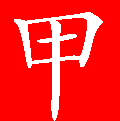
\includegraphics[width=3mm]{../Images/00002}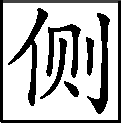
\includegraphics[width=3mm]{../Images/00011}\footnotesize \kaishu 全是体贴功夫。}因想起近日薛宝钗在家养病,未去亲候,意欲去望他一望。若从上房后角门过去,又恐遇见别事缠绕,再或可巧遇见他父亲,{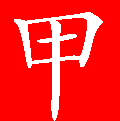
\includegraphics[width=3mm]{../Images/00002}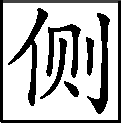
\includegraphics[width=3mm]{../Images/00011}\footnotesize \kaishu 本意正传,实是曩时苦恼,叹叹!}更为不妥,{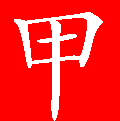
\includegraphics[width=3mm]{../Images/00002}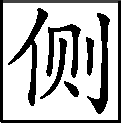
\includegraphics[width=3mm]{../Images/00011}\footnotesize \kaishu 细甚。}宁可绕远路罢了。当下众嬷嬷丫鬟伺候他换衣服,见他不换,仍出二门去了。众嬷嬷丫鬟只得跟随出来,还只当他去那府中看戏。谁知到了穿堂,便向东向北绕厅后而去。偏顶头遇见了门下清客相公詹光{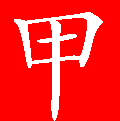
\includegraphics[width=3mm]{../Images/00002}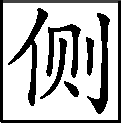
\includegraphics[width=3mm]{../Images/00011}\footnotesize \kaishu 妙!盖沾光之意。}、单聘仁{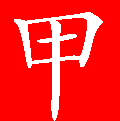
\includegraphics[width=3mm]{../Images/00002}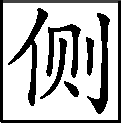
\includegraphics[width=3mm]{../Images/00011}\footnotesize \kaishu 更妙!盖善于骗人之意。}二人走来,一见了宝玉,便都笑着赶上来,一个抱住腰,一个携着手,都道:“我的菩萨哥儿,{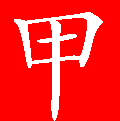
\includegraphics[width=3mm]{../Images/00002}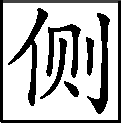
\includegraphics[width=3mm]{../Images/00011}\footnotesize \kaishu 没理没伦,口气毕肖。}我说作了好梦呢,好容易得遇见了你。”说着,请了安,又问好,唠叨了半日,方才走开。{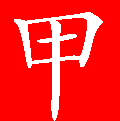
\includegraphics[width=3mm]{../Images/00002}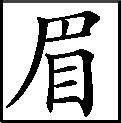
\includegraphics[width=3mm]{../Images/00010}\footnotesize \kaishu 一路用淡三色烘染、行云流水之法,写出贵公子家常不即不离气致。经历过者则喜其写真,未经者恐不免嫌繁。}老嬷嬷叫住,因问:“你二位爷是从老爷跟前来的不是?”{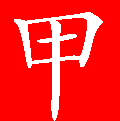
\includegraphics[width=3mm]{../Images/00002}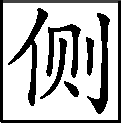
\includegraphics[width=3mm]{../Images/00011}\footnotesize \kaishu 为玉兄一人,却人人俱有心事,细致。}他二人点头道:“老爷在梦坡斋{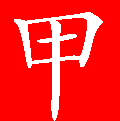
\includegraphics[width=3mm]{../Images/00002}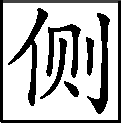
\includegraphics[width=3mm]{../Images/00011}\footnotesize \kaishu 使人起遐思。{$\diamond$}妙!梦遇坡仙之处也。}小书房里歇中觉呢,不妨事的。”{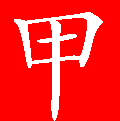
\includegraphics[width=3mm]{../Images/00002}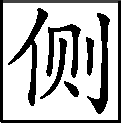
\includegraphics[width=3mm]{../Images/00011}\footnotesize \kaishu 玉兄知己。一笑。}一面说,一面走了。说的宝玉也笑了。

于是转弯向北奔梨香院来。{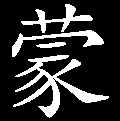
\includegraphics[width=3mm]{../Images/00006}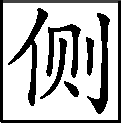
\includegraphics[width=3mm]{../Images/00011}\footnotesize \kaishu 吃冷香丸,住梨香院。有趣。}可巧银库房的总领名唤吴新登{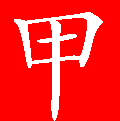
\includegraphics[width=3mm]{../Images/00002}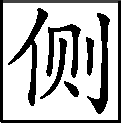
\includegraphics[width=3mm]{../Images/00011}\footnotesize \kaishu 妙!盖云无星戥也。}与仓上的头目名戴良,{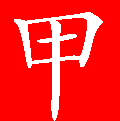
\includegraphics[width=3mm]{../Images/00002}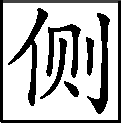
\includegraphics[width=3mm]{../Images/00011}\footnotesize \kaishu 妙!盖云大量也。}还有几个管事的头目,共有七个人,从账房里出来,一见了宝玉,赶来都一齐垂手站住。独有一个买办名唤钱华的,{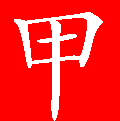
\includegraphics[width=3mm]{../Images/00002}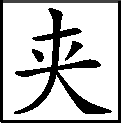
\includegraphics[width=3mm]{../Images/00012}\footnotesize \kaishu 亦钱开花之意。随事生情,因情得文。}因他多日未见宝玉,忙上来打千儿请安,宝玉忙含笑携他起来。众人都笑说:“前儿在一处看见二爷写的斗方,字法越发好了,多早晚赏我们几张贴贴。”{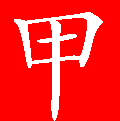
\includegraphics[width=3mm]{../Images/00002}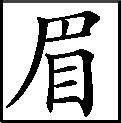
\includegraphics[width=3mm]{../Images/00010}\footnotesize \kaishu 余亦受过此骗,今阅至此,赧然一笑。此时有三十年前向余作此语之人在侧,观其形已皓首驼腰矣,乃使彼亦细听此数语,彼则潸然泣下,余亦为之败兴。}宝玉笑道:“在那里看见了?”众人道:“好几处都有,都称赞的了不得,还和我们寻呢。”{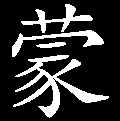
\includegraphics[width=3mm]{../Images/00006}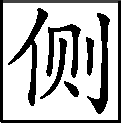
\includegraphics[width=3mm]{../Images/00011}\footnotesize \kaishu 侍奉上人者,无此等见识、无此等迎奉者,难乎免于厌弃,呜呼哀哉。}宝玉笑道:“不值什么,你们说给我的小幺儿们就是了。”一面说,一面前走,众人待他过去,方都各自散了。{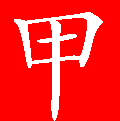
\includegraphics[width=3mm]{../Images/00002}\includegraphics[width=3mm]{../Images/00012}\footnotesize \kaishu 未入梨香院,先故作若许波澜曲折。瞧他无意中又写出宝玉写字来,固是愚弄公子闲文,然亦是暗逗宝玉历来文课事。不然,后文岂不太突?}

闲言少述,{\includegraphics[width=3mm]{../Images/00002}\includegraphics[width=3mm]{../Images/00012}\footnotesize \kaishu 此处用此句最当。}且说宝玉来至梨香院中,先入薛姨妈室中来,正见薛姨妈打点针黹与丫鬟们呢。宝玉忙请了安,薛姨妈忙一把拉了他,抱入怀内,笑说:“这么冷天,我的儿,难为你想着来,快上炕来坐着罢。”命人倒滚滚的茶来。宝玉因问:“哥哥不在家?”薛姨妈叹道:“他是没笼头的马,天天逛不了,那里肯在家一日。”宝玉道:“姐姐可大安了?”薛姨妈道:“可是呢,你前儿又想着打发人来瞧他。他在里间不是,你去瞧他。里间比这里暖和,那里坐着,我收拾收拾就进去和你说话儿。”{\includegraphics[width=3mm]{../Images/00006}\includegraphics[width=3mm]{../Images/00011}\footnotesize \kaishu 作者何等笔法。“里间里”三字,恐文气不足,又贯之以“比这里和暖”。其笔真是神龙云中弄影,是必当进去的神理。}

宝玉听说,忙下了炕,来至里间门前,只见吊着半旧的红紬软帘。{\includegraphics[width=3mm]{../Images/00002}\includegraphics[width=3mm]{../Images/00011}\footnotesize \kaishu 从门外看起,有层次。}宝玉掀帘一迈步进去,先就看见薛宝钗坐在炕上作针线,头上挽着漆黑油光的䰖儿,蜜合色棉袄,玫瑰紫二色金银鼠比肩褂,葱黄绫棉裙,一色半新不旧,看来不觉奢华。唇不点而红,眉不画而翠;脸若银盆,眼如水杏。罕言寡语,人谓藏愚;安分随时,自云守拙。{\includegraphics[width=3mm]{../Images/00002}\includegraphics[width=3mm]{../Images/00012}\footnotesize \kaishu 这方是宝卿正传。与前写黛玉之传一齐参看,各极其妙,各不相犯,使其人难其左右于毫末。 \includegraphics[width=3mm]{../Images/00002}\includegraphics[width=3mm]{../Images/00010}\footnotesize \kaishu 画神鬼易,画人物难。写宝卿正是写人之笔,若与黛玉并写更难。今作者写得一毫难处不见,且得二人真体实传,非神助而何?}宝玉一面看,一面口内问:“姐姐可大愈了?”宝钗抬头{\includegraphics[width=3mm]{../Images/00002}\includegraphics[width=3mm]{../Images/00011}\footnotesize \kaishu 与宝玉迈步针对。}只见宝玉进来,{\includegraphics[width=3mm]{../Images/00002}\includegraphics[width=3mm]{../Images/00012}\footnotesize \kaishu 此则神情尽在烟飞水逝之间,一展眼便失于千里矣。}连忙起来含笑答说:“已经大好了,倒多谢记挂着。”说着,让他在炕沿上坐了,即命莺儿斟茶来。一面又问老太太、姨妈安,别的姊妹们都好。{\includegraphics[width=3mm]{../Images/00002}\includegraphics[width=3mm]{../Images/00011}\footnotesize \kaishu 这是口中如此。}一面{\includegraphics[width=3mm]{../Images/00002}\includegraphics[width=3mm]{../Images/00011}\footnotesize \kaishu “一面”二,口中眼中,神情俱到。}看宝玉头上戴着缧丝嵌宝紫金冠,额上勒着二龙抢珠金抹额,身上穿着秋香色立蟒白狐腋箭袖,系着五色蝴蝶銮绦\footnote{銮绦”:己、庚、蒙本同,杨、列、舒本作“赤金绦”(当是误把“銮”拆作两字)。唯戚序、甲辰本作“鸾绦”。按“銮绦”不可解,鸾绦则指“束腰的丝带”,后文第三十二回又有“或玉环金佩,或鲛帕鸾绦”之语。似应以“鸾绦”为是。但“銮绦”既有各主要版本支持,究是笔误还是另有出处,存疑待考。},项上挂着长命锁、记名符,另外有那一块落草时衔下来的宝玉。

宝钗因笑说道:“成日家说你的这玉,究竟未曾细细的赏鉴,我今儿倒要瞧瞧。”{\includegraphics[width=3mm]{../Images/00002}\includegraphics[width=3mm]{../Images/00012}\footnotesize \kaishu 自首回至此,回回说有通灵玉一物,余亦未曾细细赏鉴,今亦欲一见。}说着便挪近前来。宝玉亦凑了上去,从项上摘了下来,递在宝钗手内。宝钗托于掌上,{\includegraphics[width=3mm]{../Images/00002}\includegraphics[width=3mm]{../Images/00012}\footnotesize \kaishu 试问石兄:此一托,比在青埂峰下猿啼虎啸之声何如? \includegraphics[width=3mm]{../Images/00002}\includegraphics[width=3mm]{../Images/00010}\footnotesize \kaishu 余代答曰:“遂心如意。”}只见大如雀卵,{\includegraphics[width=3mm]{../Images/00002}\includegraphics[width=3mm]{../Images/00011}\footnotesize \kaishu 体。}灿若明霞,{\includegraphics[width=3mm]{../Images/00002}\includegraphics[width=3mm]{../Images/00011}\footnotesize \kaishu 色。}莹润如酥,{\includegraphics[width=3mm]{../Images/00002}\includegraphics[width=3mm]{../Images/00011}\footnotesize \kaishu 质。}五色花纹缠护。{\includegraphics[width=3mm]{../Images/00002}\includegraphics[width=3mm]{../Images/00011}\footnotesize \kaishu 文。}这就是大荒山中青埂峰下的那块顽石的幻相。{\includegraphics[width=3mm]{../Images/00002}\includegraphics[width=3mm]{../Images/00011}\footnotesize \kaishu 注明。}后人曾有诗嘲云:

女娲炼石已荒唐,又向荒唐演大荒。

失去幽灵真境界,幻来亲就臭皮囊。{\includegraphics[width=3mm]{../Images/00002}\includegraphics[width=3mm]{../Images/00011}\footnotesize \kaishu 二语可入道,故前引庄叟秘诀。}

好知运败金无彩,{\includegraphics[width=3mm]{../Images/00002}\includegraphics[width=3mm]{../Images/00011}\footnotesize \kaishu 又夹入宝钗,不是虚图对得工。}堪叹时乖玉不光。{\includegraphics[width=3mm]{../Images/00002}\includegraphics[width=3mm]{../Images/00011}\footnotesize \kaishu 二语虽粗,本是真情,然此等诗只宜如此。为天下儿女一哭。}

白骨如山忘姓氏,无非公子与红妆。{\includegraphics[width=3mm]{../Images/00002}\includegraphics[width=3mm]{../Images/00011}\footnotesize \kaishu 批得好。末二句似与题不切,然正是极贴切语。}

那顽石亦曾记下他这幻相并癞僧所镌的篆文,今亦按图画于后。但其真体最小,方能从胎中小儿口中衔下。今若按其体画,恐字迹过于微细,使观者大废眼光,亦非畅事。故今按其形式,无非略展放些规矩,使观者便于灯下醉中可阅。今注明此故,方无“胎中之儿口有多大,怎得衔此狼犺蠢大之物”等语之谤。{\includegraphics[width=3mm]{../Images/00002}\includegraphics[width=3mm]{../Images/00010}\footnotesize \kaishu 又忽作此数语,以幻弄成真,以真弄成幻。真真假假,恣意游戏于笔墨之中,可谓狡猾之至。{$\diamond$}作人要老诚,作文要狡猾。}
\begin{figure}[htp]
	\centering
	\begin{subfigure}{12em}
	  \centering
	  \includegraphics[height=20mm]{../images/00018} %以pic.jpg的0.5倍大小输出
	  \\音注云:\parbox[t]{4em}%
		{通灵宝玉 莫失莫忘 仙寿恒昌}
	%   \end{example}
	  \caption{通灵宝玉正面图式}
	  \label{fig:subfigure-cap1}
	\end{subfigure}
	\qquad
	\begin{subfigure}{12em}
	  \centering
	  \includegraphics[height=20mm]{../images/00019}
	  \\音注云:\parbox[t]{4em}%
	  {一除邪祟 二疗冤疾 三知祸福}
	  \caption{通灵宝玉反面图式}
	  \label{fig:subfigure-cap2}
	\end{subfigure}
	% \caption{通灵宝玉}
	\label{fig:subcaption}
\end{figure}

宝钗看毕,{\includegraphics[width=3mm]{../Images/00002}\includegraphics[width=3mm]{../Images/00012}\footnotesize \kaishu 余亦想见其物矣。前回中总用草蛇灰线写法,至此方细细写出,正是大关节处。}又从翻过正面来细看,{\includegraphics[width=3mm]{../Images/00002}\includegraphics[width=3mm]{../Images/00011}\footnotesize \kaishu 可谓真奇之至。}口内念道:“莫失莫忘,仙寿恒昌。”{\includegraphics[width=3mm]{../Images/00002}\includegraphics[width=3mm]{../Images/00011}\footnotesize \kaishu 是心中沉吟,神理。 \includegraphics[width=3mm]{../Images/00002}\includegraphics[width=3mm]{../Images/00010}\footnotesize \kaishu 《石头记》立誓一笔不写一家文字。}念了两遍,乃回头向莺儿笑道:“你不去倒茶,也在这里发呆作什么?”{\includegraphics[width=3mm]{../Images/00002}\includegraphics[width=3mm]{../Images/00012}\footnotesize \kaishu 请诸公掩卷合目想其神理,想其坐立之势,想宝钗面上口中。真妙!}莺儿嘻嘻笑道:“我听这两句话,倒像和姑娘的项圈上的两句话是一对儿。”{\includegraphics[width=3mm]{../Images/00002}\includegraphics[width=3mm]{../Images/00012}\footnotesize \kaishu 又引出一个金项圈来,莺儿口中说出方妙。 \includegraphics[width=3mm]{../Images/00002}\includegraphics[width=3mm]{../Images/00010}\footnotesize \kaishu 恨颦儿不早来听此数语,若使彼闻之,不知又有何等妙论趣语以悦我等心臆。}宝玉听了,忙笑道:“原来姐姐那项圈上也有八个字,{\includegraphics[width=3mm]{../Images/00002}\includegraphics[width=3mm]{../Images/00012}\footnotesize \kaishu 补出素日眼中虽见而实未留心。}我也鉴赏鉴赏!”宝钗道:“你别听他的话,没有什么字。”宝玉笑央:“好姐姐,你怎么瞧我的呢!”宝钗被他缠不过,因说道:“是个人\footnote{按:“是个人”,己、庚、蒙、戚等本作“也是个人”。其实从说话语气来看,添这个字是没有道理的。}给了两句吉利话儿,{\includegraphics[width=3mm]{../Images/00006}\includegraphics[width=3mm]{../Images/00011}\footnotesize \kaishu “也是个”等字移换得巧妙,其雅量尊重在不言之表。}所以錾上了,叫天天带着,不然,沉甸甸的有什么趣儿。”{\includegraphics[width=3mm]{../Images/00002}\includegraphics[width=3mm]{../Images/00012}\footnotesize \kaishu 一句骂死天下浓妆艳饰富贵中之脂妖粉怪。}一面说,一面解排扣,{\includegraphics[width=3mm]{../Images/00002}\includegraphics[width=3mm]{../Images/00011}\footnotesize \kaishu 细。}从里面大红袄上{\includegraphics[width=3mm]{../Images/00006}\includegraphics[width=3mm]{../Images/00011}\footnotesize \kaishu 打开,好看煞人。}将那珠宝晶莹黄金灿烂的璎珞掏将出来。{\includegraphics[width=3mm]{../Images/00002}\includegraphics[width=3mm]{../Images/00012}\footnotesize \kaishu 按,璎珞者,颈饰也!想近俗即呼为项圈者是矣。}宝玉忙托了锁看时,果然一面有四个篆字,两面八个,共成两句吉谶。亦曾按式画下形相:
\begin{figure}[htp]
	\centering
	\begin{subfigure}{12em}
	  \centering
	  \includegraphics[height=10mm]{../images/00020} %以pic.jpg的0.5倍大小输出
	  \\音注云:\parbox[t]{4em}%
		{不离不弃}
	%   \end{example}
	  \caption{璎珞正面式}
	  \label{fig:subfigure2-cap1}
	\end{subfigure}
	\qquad
	\begin{subfigure}{12em}
	  \centering
	  \includegraphics[height=10mm]{../images/00021}
	  \\音注云:\parbox[t]{4em}%
	  {芳龄永继}
	  \caption{璎珞反面式}
	  \label{fig:subfigure2-cap2}
	\end{subfigure}
	% \caption{通灵宝玉}
	\label{fig:subcaption2}
\end{figure}
%\section{通灵宝玉正面图式}
% \begin{figure}[htbp]
% 	\centering %居中
% 	\subfigure[璎珞正面式]{ %第一张子图
% 		\begin{minipage}{5cm}
% 			\centering %子图居中
% 			\includegraphics[scale=0.335]{../images/00020} %以pic.jpg的0.5倍大小输出
% 		\end{minipage}
% 	}
% 	\subfigure[璎珞反面式]{ %第二张子图
% 		\begin{minipage}{5cm}
% 			\centering %子图居中
% 			\includegraphics[scale=0.335]{../images/00021} %以pic.jpg的0.5倍大小输出
% 		\end{minipage}
% 	}
% 	\caption{璎珞} % %大图名称
% 	\label{fig:2} %图片引用标记
% \end{figure}

{{\includegraphics[width=3mm]{../Images/00002}\includegraphics[width=3mm]{../Images/00011}\footnotesize \kaishu 合前读之,岂非一对? }\includegraphics[width=3mm]{../Images/00003}\includegraphics[width=3mm]{../Images/00012}\footnotesize \kaishu “不离不弃”与“莫失莫忘”相对,所谓愈出愈奇。{$\diamond$}“芳龄永继”又与“仙寿恒昌”一对。请合而读之。问诸公历来小说中,可有如此可巧奇妙之文,以换新眼目?}

宝玉看了,也念两遍,又念自己的两遍,因笑问:“姐姐这八个字倒真与我的是一对。”{\includegraphics[width=3mm]{../Images/00002}\includegraphics[width=3mm]{../Images/00012}\footnotesize \kaishu 余亦谓是一对,不知干支中四柱八字可与卿亦对否? \includegraphics[width=3mm]{../Images/00002}\includegraphics[width=3mm]{../Images/00010}\footnotesize \kaishu 花看半开,酒饮微醉,此文字是也。}莺儿笑道:“是个癞头和尚送的,他说必须錾在金器上\ldots{}\ldots{}”{\includegraphics[width=3mm]{../Images/00006}\includegraphics[width=3mm]{../Images/00011}\footnotesize \kaishu 和尚在幻境中作如此勾当,亦属多事。}宝钗不待说完,便嗔他不去倒茶,{\includegraphics[width=3mm]{../Images/00006}\includegraphics[width=3mm]{../Images/00011}\footnotesize \kaishu “嗔”字一截,截得妙。}一面又问宝玉从那里来。{\includegraphics[width=3mm]{../Images/00002}\includegraphics[width=3mm]{../Images/00011}\footnotesize \kaishu 妙神妙理,请观者自思。}

宝玉与宝钗相近,只闻一阵阵凉森森甜丝丝的幽香,{\includegraphics[width=3mm]{../Images/00006}\includegraphics[width=3mm]{../Images/00011}\footnotesize \kaishu 这方是花香袭人正意。}竟不知系何香气,遂问:“姐姐熏的是什么香?我竟从未闻见过这味儿。”{\includegraphics[width=3mm]{../Images/00002}\includegraphics[width=3mm]{../Images/00011}\footnotesize \kaishu 不知比“群芳髓”又何如?}宝钗笑道:“我最怕熏香,好好的衣服,熏的烟燎火气的。”{\includegraphics[width=3mm]{../Images/00002}\includegraphics[width=3mm]{../Images/00011}\footnotesize \kaishu 真真骂死一干浓妆艳饰鬼怪。}宝玉道:“既如此,这是什么香?”宝钗想了一想,笑道:“是了,是我早起吃了丸药的香气。”{\includegraphics[width=3mm]{../Images/00002}\includegraphics[width=3mm]{../Images/00011}\footnotesize \kaishu 点“冷香丸”。}宝玉笑道:“什么丸药这么好闻?好姐姐,给我一丸尝尝。”{\includegraphics[width=3mm]{../Images/00002}\includegraphics[width=3mm]{../Images/00012}\footnotesize \kaishu 仍是小儿语气。究竟不知别个小儿,只宝玉如此。}宝钗笑道:“又混闹了,一个药也是混吃的?”

一语未了,{\includegraphics[width=3mm]{../Images/00006}\includegraphics[width=3mm]{../Images/00011}\footnotesize \kaishu 每善用此等转换法。}忽听外面人说:“林姑娘来了。”{\includegraphics[width=3mm]{../Images/00002}\includegraphics[width=3mm]{../Images/00011}\footnotesize \kaishu 紧处愈紧,密不容针之文。}话犹未了,林黛玉已摇摇{\includegraphics[width=3mm]{../Images/00002}\includegraphics[width=3mm]{../Images/00011}\footnotesize \kaishu 二字画出身。}的走了进来,一见了宝玉,便笑道:“嗳哟,我来的不巧了!”{{\includegraphics[width=3mm]{../Images/00002}\includegraphics[width=3mm]{../Images/00011}\footnotesize \kaishu 奇文,我实不知颦儿心中是何丘壑。 }\includegraphics[width=3mm]{../Images/00006}\includegraphics[width=3mm]{../Images/00011}\footnotesize \kaishu 怪急语。}宝玉等忙起身笑让坐,宝钗因笑道:“这话怎么说?”{\includegraphics[width=3mm]{../Images/00006}\includegraphics[width=3mm]{../Images/00011}\footnotesize \kaishu 不得不问。}黛玉笑道:“早知他来,我就不来了。”{\includegraphics[width=3mm]{../Images/00006}\includegraphics[width=3mm]{../Images/00011}\footnotesize \kaishu 更叫人急煞。}宝钗道:“我更不解这意。”黛玉笑道:“要来时一群都来,要不来一个也不来,今儿他来了,明儿我再来,如此间错开了来着,岂不天天有人来了?{\includegraphics[width=3mm]{../Images/00002}\includegraphics[width=3mm]{../Images/00011}\footnotesize \kaishu 强词夺理。}也不至于太冷落,也不至于太热闹了。{\includegraphics[width=3mm]{../Images/00002}\includegraphics[width=3mm]{../Images/00011}\footnotesize \kaishu 好点缀。}姐姐如何反不解这意思?”{\includegraphics[width=3mm]{../Images/00002}\includegraphics[width=3mm]{../Images/00012}\footnotesize \kaishu 吾不知颦儿以何物为心为齿,为口为舌,实不知胸中有何丘壑。}

宝玉因见他外面罩着大红羽缎对衿褂子,{{\includegraphics[width=3mm]{../Images/00002}\includegraphics[width=3mm]{../Images/00011}\footnotesize \kaishu 岔开文字,{[}避{]}繁章法,妙极妙极! }\includegraphics[width=3mm]{../Images/00006}\includegraphics[width=3mm]{../Images/00011}\footnotesize \kaishu 又一转换。若无此则必有宝玉之穷究,而宝钗之重复,加长无味。此等文章是《西游记》的请观世音菩萨,菩萨一到,无不扫地完结者。}因问:“下雪了么?”地下婆娘们道:“下了这半日雪珠儿了。”宝玉道:“取了我的斗篷来了不曾?”黛玉便道:“是不是?我来了你就该去了。”{\includegraphics[width=3mm]{../Images/00002}\includegraphics[width=3mm]{../Images/00011}\footnotesize \kaishu 实不知有何丘壑。}宝玉笑道:“我多早晚说要去了?不过是拿来预备着。”宝玉的奶母李嬷嬷因说道:“天又下雪,也好早晚的了,就在这里同姐姐妹妹一处顽顽罢。姨妈那里摆茶果子呢。我叫丫头去取了斗篷来,说给小幺儿们散了罢。”宝玉应允。李嬷嬷出去,命小厮们都各散去不提。{\includegraphics[width=3mm]{../Images/00006}\includegraphics[width=3mm]{../Images/00011}\footnotesize \kaishu 极力写嬷嬷周旋,是反衬下文。}

这里薛姨妈已摆了几样细巧茶果,留他们吃茶。{\includegraphics[width=3mm]{../Images/00002}\includegraphics[width=3mm]{../Images/00011}\footnotesize \kaishu 是溺爱,非势利。}宝玉因夸前日在那府里珍大嫂子的好鹅掌、鸭信。{\includegraphics[width=3mm]{../Images/00002}\includegraphics[width=3mm]{../Images/00012}\footnotesize \kaishu 为前日秦钟之事,恐观者忘却,故忙中闲笔,重一渲染。}薛姨妈听了,忙也把自己糟的取了些来与他尝。{{\includegraphics[width=3mm]{../Images/00002}\includegraphics[width=3mm]{../Images/00011}\footnotesize \kaishu 是溺爱,非夸富。 }\includegraphics[width=3mm]{../Images/00006}\includegraphics[width=3mm]{../Images/00011}\footnotesize \kaishu 不写酒先写糟,将糟引酒。}宝玉笑道:“这个须得就酒才好。”薛姨妈便命人去灌了些上等的酒来。{\includegraphics[width=3mm]{../Images/00002}\includegraphics[width=3mm]{../Images/00011}\footnotesize \kaishu 愈见溺爱。}李嬷嬷便上来道:“姨太太,酒倒罢了。”{\includegraphics[width=3mm]{../Images/00002}\includegraphics[width=3mm]{../Images/00010}\footnotesize \kaishu 余最恨无调教之家,任其子侄肆行哺啜,观此则知大家风范。}宝玉笑央道:“好妈妈,我只吃一钟。”李嬷嬷道:“不中用!当着老太太、太太,那怕你吃一坛呢。想那日我眼错不见一会,不知是那一个没调教的,只图讨你的好儿,不管别人死活,给了你一口酒吃,葬送的我挨了两日骂。姨太太不知道,他性子又可恶,{\includegraphics[width=3mm]{../Images/00002}\includegraphics[width=3mm]{../Images/00011}\footnotesize \kaishu 补出素日。}吃了酒更弄性。有一日老太太高兴了,又尽着他吃,什么日子又不许他吃,何苦我白赔在里面。”{{\includegraphics[width=3mm]{../Images/00002}\includegraphics[width=3mm]{../Images/00011}\footnotesize \kaishu 浪酒闲茶,原不相宜。 }\includegraphics[width=3mm]{../Images/00006}\includegraphics[width=3mm]{../Images/00011}\footnotesize \kaishu 嬷嬷口气。}薛姨妈笑道:“老货,{\includegraphics[width=3mm]{../Images/00002}\includegraphics[width=3mm]{../Images/00011}\footnotesize \kaishu 二字如闻。}你只放心吃你的去。我也不许他吃多了。便是老太太问,有我呢。”一面令小丫鬟:“来,让你奶奶们去,也吃杯搪搪雪气。”那李嬷嬷听如此说,只得和众人且去吃些酒水。这里宝玉又说:“不必烫热了,我只爱吃冷的。”薛姨妈忙道:“这可使不得,吃了冷酒,写字手打飐儿。”{{\includegraphics[width=3mm]{../Images/00002}\includegraphics[width=3mm]{../Images/00011}\footnotesize \kaishu 酷肖。 }\includegraphics[width=3mm]{../Images/00006}\includegraphics[width=3mm]{../Images/00011}\footnotesize \kaishu 点石成金。}宝钗笑道:“宝兄弟,亏你每日家杂学旁收的,{\includegraphics[width=3mm]{../Images/00002}\includegraphics[width=3mm]{../Images/00011}\footnotesize \kaishu 着眼。若不是宝卿说出,竟不知玉卿日就何业。 \includegraphics[width=3mm]{../Images/00002}\includegraphics[width=3mm]{../Images/00010}\footnotesize \kaishu 在宝卿口中说出玉兄学业,是作微露卸春挂之萌耳,是书勿看正面为幸。}难道就不知道酒性最热,若热吃下去,发散的就快,若冷吃下去,便凝结在内,以五脏去暖他,岂不受害?从此还不快不要吃那冷的呢。”{\includegraphics[width=3mm]{../Images/00002}\includegraphics[width=3mm]{../Images/00012}\footnotesize \kaishu 知命知身,识理识性,博学不杂,庶可称为佳人。可笑别小说中一首歪诗,几句淫曲,便自佳人相许,岂不丑杀?}宝玉听这话有情理,{\includegraphics[width=3mm]{../Images/00002}\includegraphics[width=3mm]{../Images/00012}\footnotesize \kaishu 宝玉亦听的出有情理的话来,与前问读书家务,并皆大奇之事。}便放下冷的,命人暖来方饮。

黛玉磕着瓜子儿,只抿着嘴笑。{{\includegraphics[width=3mm]{../Images/00002}\includegraphics[width=3mm]{../Images/00011}\footnotesize \kaishu 实不知其丘壑,自何处设想而来?}\includegraphics[width=3mm]{../Images/00006}\includegraphics[width=3mm]{../Images/00011}\footnotesize \kaishu 笑的毒。}可巧{\includegraphics[width=3mm]{../Images/00002}\includegraphics[width=3mm]{../Images/00011}\footnotesize \kaishu 又用此二字。}黛玉的小丫鬟雪雁走来,与黛玉送小手炉来,黛玉因含笑问他说:“谁叫你送来的?难为他费心,那里就冷死了我!”{\includegraphics[width=3mm]{../Images/00002}\includegraphics[width=3mm]{../Images/00011}\footnotesize \kaishu 吾实不知何为心,何为齿、口、舌。}雪雁道:“紫鹃{\includegraphics[width=3mm]{../Images/00002}\includegraphics[width=3mm]{../Images/00011}\footnotesize \kaishu 鹦哥改名也。}姐姐{\includegraphics[width=3mm]{../Images/00002}\includegraphics[width=3mm]{../Images/00012}\footnotesize \kaishu 又顺笔带出一个妙名来,洗尽春花、腊梅等套。}怕姑娘冷,使我送来的。”黛玉一面接了,抱在怀中,笑道:“也亏你倒听他的话。我平日和你说的,全当耳旁风,怎么他说了你就依,比圣旨还快呢!”{{\includegraphics[width=3mm]{../Images/00002}\includegraphics[width=3mm]{../Images/00012}\footnotesize \kaishu 要知尤物方如此,莫作世俗中一味酸妒狮吼辈看去。 }\includegraphics[width=3mm]{../Images/00006}\includegraphics[width=3mm]{../Images/00011}\footnotesize \kaishu 句句尖刺,可恨可爱,而句意毫无滞碍。}宝玉听这话,知是黛玉借此奚落他,也无回复之词,只嘻嘻的笑了两阵罢了。{\includegraphics[width=3mm]{../Images/00002}\includegraphics[width=3mm]{../Images/00011}\footnotesize \kaishu 这才好,这才是宝玉。}宝钗素知黛玉是如此惯了的,也不去睬他。{\includegraphics[width=3mm]{../Images/00002}\includegraphics[width=3mm]{../Images/00011}\footnotesize \kaishu 浑厚天成,这才是宝钗。}薛姨妈因道:“你素日身子弱,禁不得冷的,他们记挂着你倒不好?”黛玉笑道:“姨妈不知道。幸亏是姨妈这里,倘或在别人家,人家岂不恼?{\includegraphics[width=3mm]{../Images/00006}\includegraphics[width=3mm]{../Images/00011}\footnotesize \kaishu 又转出此等言语,令人疼煞黛玉,敬煞作者。}好说就看的人家连个手炉也没有,巴巴的从家里送个来。不说丫头们太小心过馀,还只当我素日是这等轻狂惯了呢。”{\includegraphics[width=3mm]{../Images/00002}\includegraphics[width=3mm]{../Images/00012}\footnotesize \kaishu 用此一解,真可拍案叫绝,足见其以兰为心,以玉为骨,以莲为舌,以冰为神。真真绝倒天下之裙钗矣。}薛姨妈道:“你是个多心的,有这样想。我就没这样心。”

说话时,宝玉已是三杯过去。李嬷嬷又上来拦阻。宝玉正在心甜意洽之时,和宝黛姊妹说说笑笑的,{\includegraphics[width=3mm]{../Images/00002}\includegraphics[width=3mm]{../Images/00012}\footnotesize \kaishu 试问石兄:比当日青埂峰猿啼虎啸之声何如?}那肯不吃。宝玉只得屈意央告:“好妈妈,我再吃两钟就不吃了。”李嬷嬷道:“你可仔细老爷今儿在家,提防问你的书!”{\includegraphics[width=3mm]{../Images/00002}\includegraphics[width=3mm]{../Images/00012}\footnotesize \kaishu 不合提此话。这是李嬷嬷激醉了的,无怪乎后文。一笑。 \includegraphics[width=3mm]{../Images/00002}\includegraphics[width=3mm]{../Images/00011}\footnotesize \kaishu 不入耳之言是也。}宝玉听了此话,便心中大不自在,慢慢的放下酒,垂了头。{\includegraphics[width=3mm]{../Images/00002}\includegraphics[width=3mm]{../Images/00012}\footnotesize \kaishu 画出小儿愁蹙之状,楔紧后文。}黛玉先忙的说:“别扫大家的兴!舅舅{\includegraphics[width=3mm]{../Images/00002}\includegraphics[width=3mm]{../Images/00011}\footnotesize \kaishu 二字指贾政也。}若叫你,只说姨妈留着呢。这个妈妈,他吃了酒,又拿我们来醒脾了!”{\includegraphics[width=3mm]{../Images/00002}\includegraphics[width=3mm]{../Images/00011}\footnotesize \kaishu 这方是阿颦真意对玉卿之文。}一面悄推宝玉,使他赌气,一面悄悄的咕哝说:“别理那老货,咱们只管乐咱们的。”那李嬷嬷也素知黛玉的,因说道:“林姐儿,{\includegraphics[width=3mm]{../Images/00002}\includegraphics[width=3mm]{../Images/00011}\footnotesize \kaishu 如此之称似不通,却是老妪真心道出。}你不要助着他了。你倒劝劝他,只怕他还听些。”林黛玉冷笑道:“我为什么助着他?我也犯不着劝他。你这个妈妈太小心了,往常老太太又给他酒吃,如今在姨妈这里多吃一杯,料也不妨事。必定姨妈这里是外人,不当在这里的也未可知。”李嬷嬷听了,又是急,又是笑,{\includegraphics[width=3mm]{../Images/00002}\includegraphics[width=3mm]{../Images/00011}\footnotesize \kaishu 是认不得真,是不忍认真,是爱极颦儿、疼煞颦儿之意。}说道:“真真这林姑娘,说出一句话来,比刀子还尖。这算了什么呢。”宝钗也忍不住笑着,把黛玉腮上一拧,{\includegraphics[width=3mm]{../Images/00002}\includegraphics[width=3mm]{../Images/00011}\footnotesize \kaishu 我也欲拧。}说道:“真真这个颦丫头的一张嘴,叫人恨又不是,喜欢又不是。”{{\includegraphics[width=3mm]{../Images/00002}\includegraphics[width=3mm]{../Images/00011}\footnotesize \kaishu 可知余前批不谬。 }\includegraphics[width=3mm]{../Images/00006}\includegraphics[width=3mm]{../Images/00011}\footnotesize \kaishu 恨不是,喜不是,写尽一晌含容之量。}薛姨妈一面又说:“别怕,别怕,{\includegraphics[width=3mm]{../Images/00002}\includegraphics[width=3mm]{../Images/00011}\footnotesize \kaishu 是接前老爷问书之语。}我的儿!来了这里没好的你吃,别把这点子东西吓的存在心里,倒叫我不安。只管放心吃,都有我呢。越发吃了晚饭去,便醉了,就跟着我睡罢。”因命:“再热酒来!姨妈陪你吃两杯,可就吃饭罢。”{\includegraphics[width=3mm]{../Images/00002}\includegraphics[width=3mm]{../Images/00011}\footnotesize \kaishu 二语不失长上之体,且收拾若干文{[}字{]},千斤力量。}宝玉听了,方又鼓起兴来。

李嬷嬷因吩咐小丫头子们:“你们在这里小心着,我家去换了衣服就来,悄悄的回姨太太,别任他的性多给他吃。”{\includegraphics[width=3mm]{../Images/00006}\includegraphics[width=3mm]{../Images/00011}\footnotesize \kaishu “家去换衣服”是含酸欲怒,“悄悄回”的光景是不露怒。}说着便家去了。这里虽还有三四个婆子,都是不关痛痒的,{\includegraphics[width=3mm]{../Images/00002}\includegraphics[width=3mm]{../Images/00011}\footnotesize \kaishu 写得到。}见李嬷嬷走了,也都悄悄的自寻方便去了。只剩了两个小丫头子,乐得讨宝玉的欢喜。幸而薛姨妈千哄万哄的,只容他吃了两杯,就忙收过了。做了酸笋鸡皮汤,宝玉痛喝了两碗,吃了半碗饭碧粳粥。{\includegraphics[width=3mm]{../Images/00002}\includegraphics[width=3mm]{../Images/00011}\footnotesize \kaishu 美粥名。}一时薛、林二人也吃完了饭,又酽酽的潗上茶来,每人吃了两碗。薛姨妈方放了心。雪雁等三四个丫头已吃了饭,进来伺候。黛玉因问宝玉道:“你走不走?”{{\includegraphics[width=3mm]{../Images/00002}\includegraphics[width=3mm]{../Images/00011}\footnotesize \kaishu 妙问。 }\includegraphics[width=3mm]{../Images/00006}\includegraphics[width=3mm]{../Images/00011}\footnotesize \kaishu “走不走”,语言真是黛玉。}宝玉乜斜倦眼{\includegraphics[width=3mm]{../Images/00002}\includegraphics[width=3mm]{../Images/00011}\footnotesize \kaishu 醉意。}道:“你要走,我和你一同走。”{\includegraphics[width=3mm]{../Images/00002}\includegraphics[width=3mm]{../Images/00011}\footnotesize \kaishu 妙答。{$\diamond$}此等话,阿颦心中最乐。}黛玉听说,遂起身道:“咱们来了这一日,也该回去了。还不知那边怎么找咱们呢。”说着,二人便告辞。

小丫头忙捧过斗笠来,{\includegraphics[width=3mm]{../Images/00002}\includegraphics[width=3mm]{../Images/00011}\footnotesize \kaishu 不漏。}宝玉便把头略低一低,命他戴上。那丫头便将这大红猩毡斗笠一抖,才往宝玉头上一合,宝玉便说:“罢,罢!好蠢东西,你也轻些儿!难道没见过别人{\includegraphics[width=3mm]{../Images/00002}\includegraphics[width=3mm]{../Images/00011}\footnotesize \kaishu “别人”者,袭人、晴雯之辈也。}戴过的?让我自己戴罢!”黛玉站在炕沿上道:“罗唆什么,过来,我瞧瞧罢。”宝玉忙就近前来。黛玉用手整理,轻轻笼住束发冠,将笠沿拽在抹额之上,将那一颗核桃大的绛绒簪缨扶起,颤巍巍露于笠外。{\includegraphics[width=3mm]{../Images/00006}\includegraphics[width=3mm]{../Images/00011}\footnotesize \kaishu 知己最难逢,相逢意自同。花新水上香,花下水含红。}整理已毕,端相了端相,说道:“好了,披上斗篷罢。”{\includegraphics[width=3mm]{../Images/00002}\includegraphics[width=3mm]{../Images/00012}\footnotesize \kaishu 若使宝钗整理,颦卿又不知有多少文章。}宝玉听了,方接了斗篷披上。薛姨妈忙道:“跟你们的妈妈都还没来呢,且略等等不是。”宝玉道:“我们倒去等他们,有丫头们跟着也够了。”{\includegraphics[width=3mm]{../Images/00006}\includegraphics[width=3mm]{../Images/00011}\footnotesize \kaishu 伏笔。}薛姨妈不放心,便命两个妇女跟随他兄妹方罢。他二人道了扰,一径回至贾母房中。

贾母尚未用晚饭,知是薛姨妈处来,更加欢喜。{\includegraphics[width=3mm]{../Images/00002}\includegraphics[width=3mm]{../Images/00011}\footnotesize \kaishu 收的好极,正是写薛家母女。}因见宝玉吃了酒,遂命他自回房去歇着,不许再出来了。因命人好生看侍着。忽想起跟宝玉的人来,遂问众人:“李奶子怎么不见?”{{\includegraphics[width=3mm]{../Images/00002}\includegraphics[width=3mm]{../Images/00011}\footnotesize \kaishu 细。 }\includegraphics[width=3mm]{../Images/00006}\includegraphics[width=3mm]{../Images/00011}\footnotesize \kaishu 逼近。}众人不敢直说家去了,{\includegraphics[width=3mm]{../Images/00002}\includegraphics[width=3mm]{../Images/00011}\footnotesize \kaishu 有是事,大有是事。}只说:“才进来的,想有事才去了。”宝玉踉跄回头道:“他比老太太还受用呢,问他作什么!没有他只怕我还多活两日。”一面说,一面来至自己卧室。只见笔墨在案,{\includegraphics[width=3mm]{../Images/00002}\includegraphics[width=3mm]{../Images/00011}\footnotesize \kaishu 如此找前文最妙,且无逗榫之迹。}晴雯先接出来,笑说道:“好,好,耍我!研了那些墨,早起高兴,只写了三个字,丢下笔就走了,哄的我们等了一日。{\includegraphics[width=3mm]{../Images/00002}\includegraphics[width=3mm]{../Images/00011}\footnotesize \kaishu {[}娇{]}憨活现,余双圈不及。}快来给我写完这些墨才罢!”{\includegraphics[width=3mm]{../Images/00002}\includegraphics[width=3mm]{../Images/00011}\footnotesize \kaishu 补前文之未到。}宝玉忽然想起早起的事来,{\includegraphics[width=3mm]{../Images/00006}\includegraphics[width=3mm]{../Images/00011}\footnotesize \kaishu 娇痴婉转,自是不凡,引后文。}因笑道:“我写的那三个字在那里呢?”晴雯笑道:“这个人可醉了。你头过那府里去,嘱咐我贴在这门斗上的,这会子又这么问。我生怕别人贴坏了,{\includegraphics[width=3mm]{../Images/00002}\includegraphics[width=3mm]{../Images/00011}\footnotesize \kaishu 全是体贴一人。}我亲自爬高上梯的贴上,{\includegraphics[width=3mm]{../Images/00002}\includegraphics[width=3mm]{../Images/00011}\footnotesize \kaishu 可儿可儿。}这会子还冻的手僵冷的呢。”{
\includegraphics[width=3mm]{../Images/00002}\includegraphics[width=3mm]{../Images/00012}\footnotesize \kaishu 写晴雯,是晴雯走下来,断断不是袭人、平儿、莺儿等语气。 \includegraphics[width=3mm]{../Images/00002}\includegraphics[width=3mm]{../Images/00011}\footnotesize \kaishu 可儿可儿。}宝玉听了,笑{\includegraphics[width=3mm]{../Images/00002}\includegraphics[width=3mm]{../Images/00011}\footnotesize \kaishu 是醉笑。}道:“我忘了。你的手冷,我替你渥着。”说着便伸手携了晴雯的手,同仰首看门斗上新书的三个字。{{\includegraphics[width=3mm]{../Images/00002}\includegraphics[width=3mm]{../Images/00011}\footnotesize \kaishu 究竟不知是三个什么字,妙! \includegraphics[width=3mm]{../Images/00002}\includegraphics[width=3mm]{../Images/00010}\footnotesize \kaishu 是不作开门见山文字。 }\includegraphics[width=3mm]{../Images/00006}\includegraphics[width=3mm]{../Images/00011}\footnotesize \kaishu 何等景象,真是一幅教歌图。}

一时黛玉来了,宝玉便笑道:“好妹妹,你别撒谎,你看这三个字那一个字好?”黛玉仰头看里间门斗上,新贴了三个字,写着“绛芸轩”。{{\includegraphics[width=3mm]{../Images/00002}\includegraphics[width=3mm]{../Images/00011}\footnotesize \kaishu 出题。妙!原来是这三字。 }\includegraphics[width=3mm]{../Images/00006}\includegraphics[width=3mm]{../Images/00011}\footnotesize \kaishu 照应绛珠。}黛玉笑道:“个个都好。怎么写的这么好了?明儿也与我写一个匾。”{\includegraphics[width=3mm]{../Images/00002}\includegraphics[width=3mm]{../Images/00011}\footnotesize \kaishu 滑贼。}宝玉嘻嘻的笑道:“又哄我呢。”说着又问:“袭人姐姐呢?”{\includegraphics[width=3mm]{../Images/00002}\includegraphics[width=3mm]{../Images/00011}\footnotesize \kaishu 断不可少。}晴雯向里间炕上努嘴。{\includegraphics[width=3mm]{../Images/00002}\includegraphics[width=3mm]{../Images/00011}\footnotesize \kaishu 画。}宝玉一看,只见袭人和衣睡着在那里。宝玉笑道:“好,太渥早了些。”{\includegraphics[width=3mm]{../Images/00002}\includegraphics[width=3mm]{../Images/00011}\footnotesize \kaishu 绛芸轩中事。}因又问晴雯道:“今儿我那府里吃早饭,有一碟子豆腐皮的包子,我想着你爱吃,和珍大奶奶说了,只说我留着晚上吃,叫人送过来的,你可吃了?”晴雯道:“快别提。一送了来,我知道是我的,偏我才吃了饭,就搁在那里。{\includegraphics[width=3mm]{../Images/00006}\includegraphics[width=3mm]{../Images/00011}\footnotesize \kaishu 与颦儿抿着嘴儿笑的文字一样葫芦。}后来李奶奶来了看见,说:‘宝玉未必吃了,拿了给我孙子吃去罢。’他就叫人拿了家去了。”{{\includegraphics[width=3mm]{../Images/00002}\includegraphics[width=3mm]{../Images/00012}\footnotesize \kaishu 奶母之倚势亦是常情,奶母之昏愦亦是常情。然特于此处细写一回,与后文袭卿之酥酪遥遥一对,足见晴卿不及袭卿远矣。余谓晴有林风,袭乃钗副,真真不错。 }\includegraphics[width=3mm]{../Images/00006}\includegraphics[width=3mm]{../Images/00011}\footnotesize \kaishu 嬷嬷们托大处每每如此。}接着茜雪捧上茶来。宝玉因让:“林妹妹吃茶。”众人笑说:“林妹妹{\includegraphics[width=3mm]{../Images/00002}\includegraphics[width=3mm]{../Images/00011}\footnotesize \kaishu 三字是接上文口气而来,非众人之称。{$\diamond$}醉态逼真。}早走了,还让呢。”{\includegraphics[width=3mm]{../Images/00002}\includegraphics[width=3mm]{../Images/00010}\footnotesize \kaishu 写颦儿去,如此章法从何设想?奇笔奇文。}

宝玉吃了半碗茶,忽又想起早起的茶来,{\includegraphics[width=3mm]{../Images/00002}\includegraphics[width=3mm]{../Images/00012}\footnotesize \kaishu 偏是醉人搜寻的出,细事,亦是真情。}因问茜雪道:“早起潗了一碗枫露茶,{\includegraphics[width=3mm]{../Images/00002}\includegraphics[width=3mm]{../Images/00011}\footnotesize \kaishu 与“千红一窟”遥映。}我说过,那茶是三四次后才出色的,这会子怎么又潗了这个来?”{\includegraphics[width=3mm]{../Images/00002}\includegraphics[width=3mm]{../Images/00011}\footnotesize \kaishu 所谓闲茶是也,与前浪酒一般起落。}茜雪道:“我原是留着的,那会子李奶奶来了,他要尝尝,就给他吃了。”{\includegraphics[width=3mm]{../Images/00002}\includegraphics[width=3mm]{../Images/00011}\footnotesize \kaishu 又是李嬷,事有凑巧,如此类是。}宝玉听了,将手中的茶杯只顺手{\includegraphics[width=3mm]{../Images/00002}\includegraphics[width=3mm]{../Images/00011}\footnotesize \kaishu 是醉后,故用二字,非有心动气也。}往地下一掷,{\includegraphics[width=3mm]{../Images/00002}\includegraphics[width=3mm]{../Images/00010}\footnotesize \kaishu 按警幻情榜,宝玉系“情不情”。凡世间之无知无识,彼俱有一痴情去体贴。今加“大醉”二字于石兄,是因问包子、问茶、顺手掷杯、问茜雪、撵李嬷,乃一部中未有第二次事也。袭人数语,无言而止,石兄真大醉也。{$\diamond$}余亦云实实大醉也。难辞醉闹,非薛蟠纨绔辈可比!}“豁啷”一声,打个齑粉,泼了茜雪一裙子的茶。又跳起来问着茜雪道:“他是你那一门子的奶奶,你们这么孝敬他?不过是仗着我小时候吃过他几日奶罢了。{\includegraphics[width=3mm]{../Images/00002}\includegraphics[width=3mm]{../Images/00011}\footnotesize \kaishu 真醉了。}如今逞的他比祖宗还大了。如今我又吃不着奶了,白白的养着祖宗作什么!撵了出去,大家干净!”{\includegraphics[width=3mm]{../Images/00002}\includegraphics[width=3mm]{../Images/00011}\footnotesize \kaishu 真真大醉了。}说着立刻便要去回贾母,撵他乳母。

原来袭人实未睡着,不过故意装睡,引宝玉来怄他顽耍。{\includegraphics[width=3mm]{../Images/00006}\includegraphics[width=3mm]{../Images/00011}\footnotesize \kaishu 只须郎看,不禁郎嗔,是妙法。}先闻得说字、问包子等事,也还可不必起来,后来摔了茶钟,动了气,遂连忙起来解释劝阻。早有贾母遣人来问是怎么了。{\includegraphics[width=3mm]{../Images/00002}\includegraphics[width=3mm]{../Images/00011}\footnotesize \kaishu 断不可少之文。}袭人忙道:“我才倒茶来,被雪滑倒了,{{\includegraphics[width=3mm]{../Images/00002}\includegraphics[width=3mm]{../Images/00011}\footnotesize \kaishu 现成之至,瞧他写袭卿为人。 }\includegraphics[width=3mm]{../Images/00006}\includegraphics[width=3mm]{../Images/00011}\footnotesize \kaishu 袭人另有一段居心,一番行止。}失了手砸了钟子。”一面又安慰宝玉道:“你立意要撵他也好,{\includegraphics[width=3mm]{../Images/00002}\includegraphics[width=3mm]{../Images/00011}\footnotesize \kaishu 二字奇,使人一惊。}我们也都愿意出去,{\includegraphics[width=3mm]{../Images/00006}\includegraphics[width=3mm]{../Images/00011}\footnotesize \kaishu 先主取西川,方得立基业,而偏不肯取,大与此意同。}不如趁势连我们一齐撵了,我们也好,你也不愁再有好的来伏侍你。”宝玉听了这话,方无了言语,被袭人等扶至炕上,脱换了衣服。不知宝玉口内还说些什么,只觉口齿绵缠,眼眉愈加饧涩,{\includegraphics[width=3mm]{../Images/00002}\includegraphics[width=3mm]{../Images/00011}\footnotesize \kaishu 二字带出平素形象。}忙伏侍他睡下。袭人伸手从他项上摘下那通灵玉来,用自己的手帕包好,塞在褥下,次日戴时便冰不着脖子。{\includegraphics[width=3mm]{../Images/00002}\includegraphics[width=3mm]{../Images/00012}\footnotesize \kaishu 试问石兄:此一渥,比青埂峰下松风明月如何?}那宝玉就枕便睡着了。彼时李嬷嬷等已进来了,听见醉了,不敢前来再加触犯,只悄悄的打听睡了,方放心散去。{\includegraphics[width=3mm]{../Images/00002}\includegraphics[width=3mm]{../Images/00011}\footnotesize \kaishu 交代清楚。“塞玉”一段,又为“误窃”一回伏线。晴雯茜雪二婢,又为后文先作一引。 \includegraphics[width=3mm]{../Images/00002}\includegraphics[width=3mm]{../Images/00010}\footnotesize \kaishu 偷度金针法,最巧。}

次日醒来,{\includegraphics[width=3mm]{../Images/00002}\includegraphics[width=3mm]{../Images/00012}\footnotesize \kaishu 以上已完正题,以下是后文引子,前文之馀波。此回收法与前数回不同矣。}就有人回:“那边小蓉大爷带了秦相公来拜。”宝玉忙接了出去,领了拜见贾母。贾母见秦钟形容标致,举止温柔,堪陪宝玉读书,{\includegraphics[width=3mm]{../Images/00002}\includegraphics[width=3mm]{../Images/00011}\footnotesize \kaishu 娇养如此,溺爱如此。}心中十分欢喜,便留茶留饭,又命人带去见王夫人等。众人因素爱秦氏,今见了秦钟是这般人品,也都欢喜,临去时都有表礼。贾母又与了一个荷包并一个金魁星,{\includegraphics[width=3mm]{../Images/00002}\includegraphics[width=3mm]{../Images/00010}\footnotesize \kaishu 作者今尚记金魁星之事乎?抚今思昔,肠断心摧。}取“文星和合”之意。{\includegraphics[width=3mm]{../Images/00006}\includegraphics[width=3mm]{../Images/00011}\footnotesize \kaishu 雅致。}又嘱咐他道:“你家住的远,一时寒热饥饱不便,只管住在我这里,不必限定了。只和你宝叔在一处,别跟着那起不长进的东西学。”{\includegraphics[width=3mm]{../Images/00002}\includegraphics[width=3mm]{../Images/00011}\footnotesize \kaishu 总伏后文。}秦钟一一答应,回去禀知他父亲秦业。{\includegraphics[width=3mm]{../Images/00002}\includegraphics[width=3mm]{../Images/00012}\footnotesize \kaishu 妙名。业者,孽也,盖云情因孽而生也。}

这秦业现任营缮郎,{\includegraphics[width=3mm]{../Images/00002}\includegraphics[width=3mm]{../Images/00012}\footnotesize \kaishu 官职更妙,设云因情孽而缮此一书之意。}年近七十,夫人早亡。因当年无儿女,便向养生堂抱了一个儿子并一个女儿。谁知儿子又死了,{\includegraphics[width=3mm]{../Images/00002}\includegraphics[width=3mm]{../Images/00011}\footnotesize \kaishu 一顿。}只剩女儿,小名唤可儿,{\includegraphics[width=3mm]{../Images/00002}\includegraphics[width=3mm]{../Images/00012}\footnotesize \kaishu 出名。秦氏究竟不知系出何氏,所谓寓褒贬、别善恶是也。秉刀斧之笔、具菩萨之心亦甚难矣。{$\diamond$}如此写出可儿来历亦甚苦矣。又知作者是欲天下人共来哭此情字。 \includegraphics[width=3mm]{../Images/00002}\includegraphics[width=3mm]{../Images/00010}\footnotesize \kaishu 写可儿出身自养生堂,是褒中贬。后死封龙禁尉,是贬中褒。灵巧一至于此。}长大时,生得形容袅娜,性格风流。{\includegraphics[width=3mm]{../Images/00002}\includegraphics[width=3mm]{../Images/00011}\footnotesize \kaishu 四字便有隐意。《春秋》字法。}因素与贾家有些瓜葛,故结了亲,许与贾蓉为妻。那秦业五旬之上方得了秦钟。因去岁业师亡故,未暇延请高明之士,只暂在家温习旧课。正思要和亲家{\includegraphics[width=3mm]{../Images/00002}\includegraphics[width=3mm]{../Images/00011}\footnotesize \kaishu 指贾珍。}去商议,送往他家塾中,暂且不致荒废,可巧遇见了宝玉这个机会。又知贾家塾中现今司塾的是贾代儒,{\includegraphics[width=3mm]{../Images/00002}\includegraphics[width=3mm]{../Images/00011}\footnotesize \kaishu 随笔命名,省事。}乃当今之老儒,秦钟此去,学业料必进益,成名可望,因此十分欢喜。只是宦囊羞涩,那贾府上上下下都是一双富贵眼睛,{\includegraphics[width=3mm]{../Images/00002}\includegraphics[width=3mm]{../Images/00011}\footnotesize \kaishu 为天下读书人一哭、寒素人一哭。}容易拿不出来,又恐误了儿子的终身大事,{\includegraphics[width=3mm]{../Images/00002}\includegraphics[width=3mm]{../Images/00011}\footnotesize \kaishu 原来读书是终身大事。}说不得东拼西凑的恭恭敬敬{\includegraphics[width=3mm]{../Images/00002}\includegraphics[width=3mm]{../Images/00011}\footnotesize \kaishu 四字可思,近之鄙薄师傅者来看。}封了二十四两贽见礼,{{\includegraphics[width=3mm]{../Images/00002}\includegraphics[width=3mm]{../Images/00012}\footnotesize \kaishu 可知“宦囊羞涩”与“东拼西凑”等样,是特为近日守钱虏而不使子弟读书之辈一大哭。 }\includegraphics[width=3mm]{../Images/00006}\includegraphics[width=3mm]{../Images/00011}\footnotesize \kaishu 父母之恩,昊天罔极。}亲自带了秦钟,来代儒家拜见了。然后听宝玉上学之日,好一同入塾。{\includegraphics[width=3mm]{../Images/00002}\includegraphics[width=3mm]{../Images/00012}\footnotesize \kaishu 不想浪酒闲茶一段金玉旖旎之文后,忽用此等寒瘦古拙之词收住,亦行文之大变体处。《石头记》多用此法,历观后文便知。}正是:

早知日后闲争气,岂肯今朝错读书。{\includegraphics[width=3mm]{../Images/00002}\includegraphics[width=3mm]{../Images/00011}\footnotesize \kaishu 这是隐语微词,岂独指此一事哉?{$\diamond$}余则谓读书正为争气。但此“争气”与彼“争气”不同。写来一笑。}

{\includegraphics[width=3mm]{../Images/00005}\kaishu 总评:一是先天衔来之玉,一是后天造就之金。金玉相合,是成万物之象。再遇水而过寒,虽有酒浆,岂能助火?因生出黛玉之讽刺,李嬷嬷之唠叨,晴雯、茜雪之嗔恼。故不得不收功静息,涵养性天,以待再举。识丹道者,当解吾意。}

%{\label{label-2}{\ding{172}}“銮绦”:己、庚、蒙本同,杨、列、舒本作“赤金绦”(当是误把“銮”拆作两字)。唯戚序、甲辰本作“鸾绦”。按“銮绦”不可解,鸾绦则指“束腰的丝带”,后文第三十二回又有“或玉环金佩,或鲛帕鸾绦”之语。似应以“鸾绦”为是。但“銮绦”既有各主要版本支持,究是笔误还是另有出处,存疑待考。}

%{\label{label-3}{\ding{173}}按:“是个人”,己、庚、蒙、戚等本作“也是个人”。其实从说话语气来看,添这个字是没有道理的。}
%end{document}怪不得到这就结束了